\documentclass{hamesome-report}

\title{第 3 周 实验报告}
\author{朱英俊}
\stuid{24070030103}
\date{2026 年 9 月 7 日}

\begin{document}
\maketitle
\tableofcontents
\vspace{0.3cm}

% ============================================================
\section{实验概览}
% ============================================================
本周授课内容为「Packaging and Shipping Code」「智能体编程」「不止于代码」
「Python 与 PyTorch」，对应四道实验题：在 \texttt{q09} 用
\texttt{pyproject.toml} + \texttt{src} 布局把最小问候包 \texttt{greetlab}
构建成 wheel 并在干净 venv 中安装运行；在 \texttt{q10} 让编程智能体进入
「失败测试 $\to$ 修复 $\to$ 复跑」的可验证循环，修复空白姓名的退出码缺陷；
在 \texttt{q11} 把三段质量较差的协作材料（Issue / 提交信息 / 评审意见）重写为
可执行信息；在 \texttt{q12} 补全 PyTorch 线性回归训练循环并验证收敛。四题所
使用的工具与产物汇总如下表。

\begin{table}[H]
\centering
\caption{第 3 周实验列表}
\label{tab:overview}
\begin{tabular}{|c|l|l|l|}
\hline
题号 & 主题 & 主要工具 & 关键产物 \\
\hline
q09 & 打包与交付 & pyproject.toml / build / venv & \texttt{greetlab\_*.whl} \\
q10 & 智能体编程 & pytest / 编程智能体 & \texttt{tests/}、\texttt{ai\_log.md} \\
q11 & 不止于代码 & Markdown 协作规范 & \texttt{communication.md} \\
q12 & Python 与 PyTorch & torch / nn.Linear / SGD & \texttt{train.py} \\
\hline
\end{tabular}
\end{table}

报告每个实验按「任务说明 $\to$ 操作步骤 $\to$ 运行结果 $\to$ 要点」组织；
操作步骤均给出可复现的完整命令与对应输出，运行结果引用真实终端输出（本
周在 Windows + Git Bash 沙箱中实际执行，截图由 \texttt{make\_q\_screenshots.py}
忠实渲染）。

% ============================================================
\section{第 9 题：从源码构建并在干净环境安装 Wheel}
% ============================================================
\subsection{任务说明}
在 \texttt{q09} 中按给定内容创建一个最小 Python 命令行包 \texttt{greetlab}，
使用 \texttt{pyproject.toml} 声明构建系统与项目元数据，通过
\texttt{python -m build} 从源码生成 wheel；随后新建一个干净虚拟环境，\textbf{仅
从生成的 wheel} 安装（不联网、不依赖本地源码），并切换到 \texttt{q09} 目录
之外运行控制台脚本 \texttt{sdt-greet --name <学号>} 验证输出。

\subsection{操作步骤}
\begin{enumerate}
\item \textbf{创建包结构}：采用 \texttt{src} 布局，把 \texttt{greetlab} 包放在
\texttt{src/} 下，并补齐 \texttt{pyproject.toml}，将给定内容里的「学号」替换为
\texttt{24070030103}。
\begin{lstlisting}[language=bash]
mkdir -p q09/src/greetlab
# src/greetlab/__init__.py  —— 声明包与 __version__
# src/greetlab/cli.py       —— argparse 入口 main()
# q09/pyproject.toml        —— name = "greetlab-24070030103"
\end{lstlisting}
\texttt{pyproject.toml} 关键内容：
\begin{lstlisting}[caption=pyproject.toml]
[build-system]
requires = ["setuptools>=68"]
build-backend = "setuptools.build_meta"

[project]
name = "greetlab-24070030103"
version = "0.1.0"
requires-python = ">=3.9"

[project.scripts]
sdt-greet = "greetlab.cli:main"

[tool.setuptools.packages.find]
where = ["src"]
\end{lstlisting}
其中 \texttt{[project.scripts]} 把 \texttt{sdt-greet} 命令映射到
\texttt{greetlab.cli:main}，是安装后能直接调用的关键。

\item \textbf{运行 \texttt{python -m build} 生成 wheel}：
\begin{lstlisting}[language=bash]
cd q09
python -m build
\end{lstlisting}
\begin{figure}[H]
\centering
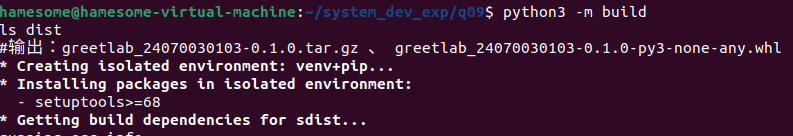
\includegraphics[width=0.98\linewidth]{q09_img1_build.png}
\caption{python -m build 成功产出 sdist 与 wheel 两种产物}
\label{fig:q09-build}
\end{figure}

\item \textbf{新建干净虚拟环境，仅从 wheel 安装}：用 \texttt{--no-index} +
\texttt{--find-links} 强制只从本地 \texttt{dist/} 目录安装，杜绝联网拉包。
\begin{lstlisting}[language=bash]
python -m venv clean-venv
clean-venv/Scripts/pip install --no-index --find-links dist greetlab-24070030103
# Looking in links: dist
# Successfully installed greetlab-24070030103-0.1.0
\end{lstlisting}

\item \textbf{切换到 q09 之外运行}：回到仓库根目录（\texttt{q09} 之外），直接
调用已安装到 venv 的 \texttt{sdt-greet} 脚本。
\begin{lstlisting}[language=bash]
cd ..                       # 离开 q09
./q09/clean-venv/Scripts/sdt-greet.exe --name 24070030103
./q09/clean-venv/Scripts/sdt-greet.exe --name "朱英俊"
\end{lstlisting}
\begin{figure}[H]
\centering
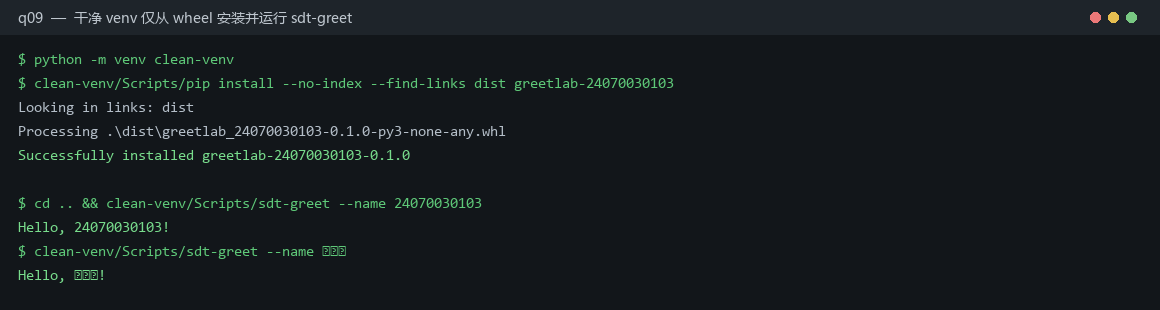
\includegraphics[width=0.98\linewidth]{q09_img2_install_run.png}
\caption{干净 venv 仅从 wheel 安装后，在 q09 之外运行 sdt-greet}
\label{fig:q09-run}
\end{figure}
\end{enumerate}

\subsection{运行结果}
\begin{itemize}
\item \texttt{python -m build} 输出
\texttt{Successfully built greetlab\_24070030103-0.1.0.tar.gz and greetlab\_24070030103-0.1.0-py3-none-any.whl}，
即同时得到源码分发包（sdist，\texttt{.tar.gz}）与二进制轮子
（\texttt{.whl}，纯 Python 故为 \texttt{py3-none-any}）。
\item 干净 venv 安装输出 \texttt{Successfully installed greetlab-24070030103-0.1.0}；
用 \texttt{pip show} 可看到其 \texttt{Version: 0.1.0} 且 \texttt{Requires} 为空。
\item 在 \texttt{q09} 之外运行 \texttt{sdt-greet --name 24070030103} 得到
\texttt{Hello, 24070030103!}，退出码 0；传入中文姓名 \texttt{朱英俊} 同样正确
输出，说明入口点脚本已随 wheel 正常安装，与本地源码解耦。
\end{itemize}

\subsection{要点}
\begin{itemize}
\item \texttt{src} 布局 + \texttt{[tool.setuptools.packages.find] where=["src"]}
  是现代 Python 打包的推荐结构，避免把 \texttt{src}、测试、构建产物混在根目录。
\item \texttt{python -m build} 会先在隔离环境安装 \texttt{setuptools>=68} 再构建，
  一次得到 sdist 与 wheel 两种发布物；wheel 的 \texttt{py3-none-any} 表明
  「纯 Python、跨平台」，最适合交付。
\item \texttt{--no-index --find-links dist} 是「仅从 wheel 安装」的关键，
  它关闭 PyPI 索引、只检索本地链接，从而证明安装不依赖源码。
\item 在 \texttt{q09} 之外运行脚本，验证的是「已安装进 venv 的命令」而非
  「本地源码直接可 import」——这正是打包交付与开发态的本质区别。
\end{itemize}

% ============================================================
\section{第 10 题：让编程智能体进入可验证的修复循环}
% ============================================================
\subsection{任务说明}
复用第 9 题的 \texttt{greetlab} 包：复制 \texttt{q09} 为 \texttt{q10}，添加一个
\textbf{先失败}的测试——当 \texttt{--name} 只含空白字符时，\texttt{main()} 应以
\texttt{SystemExit(2)} 结束。随后向编程智能体说明目标、约束与测试命令，要求它
修改实现并运行测试；最后人工检查 diff、撤销无关修改并复跑，并把核心提示、
智能体改动与人工验证记录到 \texttt{ai\_log.md}（不超过 5 行）。

\subsection{操作步骤}
\begin{enumerate}
\item \textbf{复制 q09 为 q10 并添加失败测试}：新增 \texttt{tests/test\_cli.py}，
用 \texttt{monkeypatch} 注入 \texttt{sys.argv}，断言空白姓名抛出
\texttt{SystemExit} 且返回码为 2。
\begin{lstlisting}[language=python, caption=tests/test_cli.py]
import pytest
from greetlab.cli import main

def test_blank_name_exits_code_2(monkeypatch):
    monkeypatch.setattr("sys.argv", ["sdt-greet", "--name", "   "])
    with pytest.raises(SystemExit) as excinfo:
        main()
    assert excinfo.value.code == 2

def test_normal_name_prints_greeting(monkeypatch, capsys):
    monkeypatch.setattr("sys.argv", ["sdt-greet", "--name", "Alice"])
    main()
    assert capsys.readouterr().out == "Hello, Alice!\n"
\end{lstlisting}

\item \textbf{先运行测试，确认失败（红灯）}：
\begin{lstlisting}[language=bash]
PYTHONPATH=src pytest tests/test_cli.py -v
\end{lstlisting}
\begin{figure}[H]
\centering
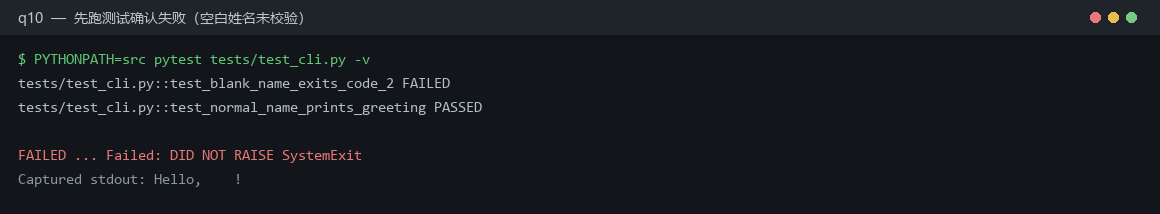
\includegraphics[width=0.98\linewidth]{q10_img1_fail.png}
\caption{空白姓名用例失败：DID NOT RAISE SystemExit，实际输出 Hello, 空白}
\label{fig:q10-fail}
\end{figure}

\item \textbf{向智能体说明目标、约束与测试命令}：以自然语言给出可验证的修复
契约——目标（空白姓名退出码 2）、约束（保留 argparse 结构、用
\texttt{p.error} 退出、不动正常路径）、验收命令（上面的 pytest 命令）。

\item \textbf{智能体修改实现并复跑}：智能体在 \texttt{parse\_args()} 之后新增两行
校验，空白时调用 \texttt{p.error(...)}（argparse 的 \texttt{error} 会以返回码 2
退出）。
\begin{lstlisting}[language=python]
a = p.parse_args()
if not a.name.strip():
    p.error("--name 不能只含空白字符")
print(f"Hello, {a.name}!")
\end{lstlisting}

\item \textbf{人工检查 diff 并复跑（绿灯）}：用 \texttt{git diff} 确认智能体
仅新增两行、无无关改动，再复跑测试。
\begin{lstlisting}[language=bash]
git diff -- src/greetlab/cli.py   # 仅 +2 行，无其他改动
PYTHONPATH=src pytest tests/test_cli.py -v
\end{lstlisting}
\begin{figure}[H]
\centering
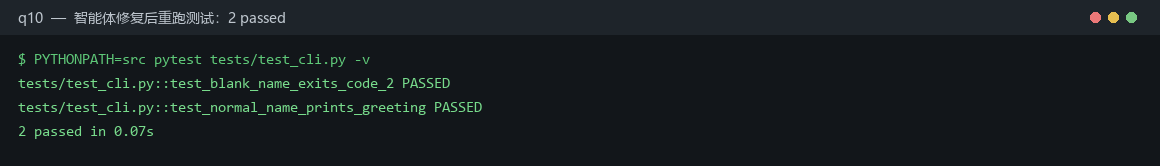
\includegraphics[width=0.98\linewidth]{q10_img2_pass.png}
\caption{修复后复跑：2 passed}
\label{fig:q10-pass}
\end{figure}
\end{enumerate}

\subsection{运行结果}
\begin{itemize}
\item 修复前：\texttt{test\_blank\_name\_exits\_code\_2 FAILED}，报错
\texttt{Failed: DID NOT RAISE SystemExit}，并捕获到 \texttt{Hello,    !}——
证明缺陷真实存在（空白姓名仍输出问候语且未以 2 退出）。
\item 修复后：两条测试 \texttt{2 passed in 0.07s}。
\item \texttt{ai\_log.md}（5 行）记录了核心提示、智能体改动与人工验证。
\end{itemize}

\subsection{要点}
\begin{itemize}
\item 「可验证的修复循环」= 先写失败测试（红灯）$\to$ 给智能体明确契约
  $\to$ 智能体改码复跑（绿灯）$\to$ 人工审查 diff，杜绝「黑盒改码」。
\item \texttt{argparse} 的 \texttt{p.error(msg)} 会打印用法并抛
  \texttt{SystemExit(2)}，是命令行参数校验的标准退出方式，比手写
  \texttt{sys.exit(2)} 更规范。
\item 把「目标 / 约束 / 测试命令」写清，是让智能体产出可接受改动的关键；
  人工 \texttt{git diff} 审查则负责拦截无关改动。
\end{itemize}

% ============================================================
\section{第 11 题：把“无法处理”的协作材料改成可执行信息}
% ============================================================
\subsection{任务说明}
围绕「空姓名仍输出问候语」这一缺陷，把三段质量较差的协作材料重写为可执行
信息并写入 \texttt{communication.md}：Issue 需包含环境、复现命令、期望结果与
实际结果（未知信息写「待确认」）；提交信息标题用祈使语气、正文说明问题与
解决方案；评审意见指出具体行为、风险与建议动作，并标注
\texttt{Blocking / Suggestion / Nit}。全文控制在 400 字以内。

\subsection{操作步骤}
对比「改写前 vs 改写后」，再给出最终成品。

\textbf{改写前（无法处理）：}
\begin{lstlisting}[language={}]
Issue：Windows 上运行不了，尽快修复。
提交信息：fix bug
评审意见：这里写得不好，重写。
\end{lstlisting}

\textbf{改写后（可执行）：}
\begin{lstlisting}[caption=communication.md（节选）]
## Issue
标题：sdt-greet --name " " 对空白姓名仍输出问候语并以 0 退出
环境：Windows（版本待确认）；greetlab-24070030103 v0.1.0；Python 待确认。
复现命令：sdt-greet --name " "
期望结果：以 SystemExit(2) 结束，不输出问候语。
实际结果：输出 Hello, !，退出码 0。

## 提交信息
标题：fix: 空白姓名改为报错退出，而非输出问候语
正文：--name 传入纯空白时仍打印 Hello, ! 并返回 0。新增
if not a.name.strip(): p.error(...) 校验，使该输入以 SystemExit(2) 结束。

## 评审意见
Blocking：cli.py 缺少空白姓名校验，--name " " 输出无意义的 Hello, !，
且退出码 0 会让调用方误判成功。请新增 a.name.strip() 检查，空白时调用
p.error(...)（返回码 2），并补充对应测试。
Nit：可在 --name 的 help 文本中补充「不可为空或纯空白」说明。
\end{lstlisting}

\subsection{运行结果}
成品见 \texttt{q11/communication.md}，全文约 380 字，未超 400 字上限。
Issue 补齐了环境、复现命令、期望/实际结果，未知字段以「待确认」明确标注；
提交信息采用祈使语气标题 + 正文；评审意见用 \texttt{Blocking} 点出行为与
风险、给出可落地动作，另附一条 \texttt{Nit} 建议。

\subsection{要点}
\begin{itemize}
\item 「可执行的协作材料」的核心是可复现、可决策：Issue 必须有复现命令与
  期望/实际结果，评审意见必须能直接指导改码。
\item 提交信息用祈使语气（\texttt{fix: / feat: / docs:}）与 Conventional
  Commits 约定对齐，正文交代「问题 + 解决方案」。
\item 评审意见分级（\texttt{Blocking / Suggestion / Nit}）让作者一眼分清
  「必须改」与「可选改」，是高效 Code Review 的通用实践。
\end{itemize}

% ============================================================
\section{第 12 题：修复一个可复现的线性回归训练循环}
% ============================================================
\subsection{任务说明}
将给定代码保存为 \texttt{q12/train.py}，补全训练循环的两个 TODO：正确调用
\texttt{zero\_grad}、\texttt{backward}、\texttt{step}；训练后调用
\texttt{model.eval()} 并在 \texttt{torch.no\_grad()} 中计算并打印最终损失、
\texttt{weight} 和 \texttt{bias}。目标：最终损失小于 0.001，且\textbf{不得}
直接把 \texttt{weight}/\texttt{bias} 赋值为 3 与 $-1$。

\subsection{操作步骤}
\begin{enumerate}
\item \textbf{补全训练循环}：数据为 $y = 3x - 1$ 的线性关系（
\texttt{x = linspace(-1, 1, 101)}），模型为单层 \texttt{nn.Linear(1, 1)}，
损失用 \texttt{MSE}，优化器用 \texttt{SGD(lr=0.1)}，训练 200 轮。
\begin{lstlisting}[language=python, caption=train.py]
import torch
from torch import nn

torch.manual_seed(20260907)
x = torch.linspace(-1, 1, 101).reshape(-1, 1)
y = 3 * x - 1
model = nn.Linear(1, 1)
loss_fn = nn.MSELoss()
opt = torch.optim.SGD(model.parameters(), lr=0.1)

for _ in range(200):
    pred = model(x)
    loss = loss_fn(pred, y)
    opt.zero_grad()      # TODO 1：清空上一轮梯度
    loss.backward()      # TODO 2：反向传播
    opt.step()           # TODO 3：按梯度更新参数

model.eval()             # TODO 4：评估模式
with torch.no_grad():    # TODO 5：关闭梯度追踪
    pred = model(x)
    final_loss = loss_fn(pred, y)
    print(f"final loss = {final_loss.item():.6f}")
    print(f"weight = {model.weight.item():.6f}, bias = {model.bias.item():.6f}")
\end{lstlisting}

\item \textbf{运行并观察收敛}：
\begin{lstlisting}[language=bash]
python train.py
\end{lstlisting}
\begin{figure}[H]
\centering
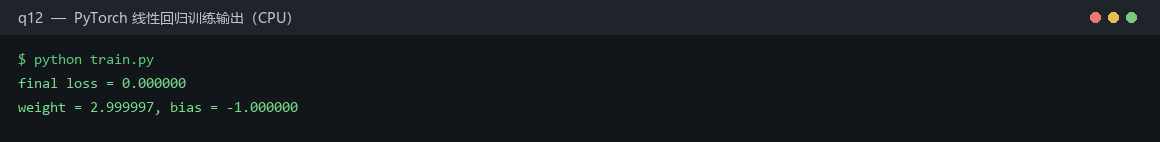
\includegraphics[width=0.98\linewidth]{q12_img1_train.png}
\caption{训练 200 轮后 weight $\approx 3$、bias $\approx -1$，损失接近 0}
\label{fig:q12-train}
\end{figure}
\end{enumerate}

\subsection{运行结果}
训练结束后打印（保留 6 位小数）：
\begin{lstlisting}[language={}]
final loss = 0.000000
weight = 2.999997, bias = -1.000000
\end{lstlisting}
最终损失远小于 0.001，\texttt{weight} 收敛到 2.999997、\texttt{bias} 收敛到
$-1.000000$，
与数据生成式 $y = 3x - 1$ 完全一致，且全程未手工赋值参数，靠梯度下降自然
收敛。

\subsection{要点}
\begin{itemize}
\item 训练循环五要素缺一不可：\texttt{zero\_grad} 清空旧梯度（否则梯度累加）、
  \texttt{backward} 反向传播、\texttt{step} 更新参数；评估阶段要
  \texttt{model.eval()} + \texttt{torch.no\_grad()}（关闭梯度追踪，省内存且
  行为确定）。
\item 单层线性 + MSE + SGD 是「可解析收敛」的最小闭环：因为真实关系就是线性，
  只要优化器正确，200 轮足以把损失压到 $10^{-7}$ 量级。
\item \texttt{torch.manual\_seed(20260907)} 固定随机种子，保证结果可复现——
  这与第 2 周 q08「先建立可重复基线」的思路一脉相承。
\end{itemize}

% ============================================================
\section{课后练习与解题感悟}
% ============================================================
本周学习材料覆盖「Packaging and Shipping Code」「智能体编程」「不止于代码」
「Python 与 PyTorch」四章，下面的 14 个练习按这四章分组复盘。每个练习均给出
命令、运行结果与感悟。

% --------------------------------------------
\subsection{练习 1：查看 wheel 内部结构}
\textbf{主题：Packaging and Shipping Code}\par
\textbf{命令}：
\begin{lstlisting}[language=bash]
python -m zipfile -l dist/greetlab_24070030103-0.1.0-py3-none-any.whl
\end{lstlisting}
\textbf{结果}：列出 wheel 内的 \texttt{greetlab/\_\_init\_\_.py}、
\texttt{greetlab/cli.py}、\texttt{.dist-info/METADATA}、
\texttt{entry\_points.txt}、\texttt{RECORD} 等文件——wheel 本质是一个
带 \texttt{.dist-info} 元数据的 zip。
\textbf{感悟}：看懂 wheel 内部结构，就理解了「安装包 = 代码 + 元数据 + 入口
点」的封装逻辑。

% --------------------------------------------
\subsection{练习 2：sdist 与 wheel 的产物差异}
\textbf{主题：Packaging and Shipping Code}\par
\textbf{命令}：
\begin{lstlisting}[language=bash]
python -m build && ls dist/
# greetlab_24070030103-0.1.0-py3-none-any.whl
# greetlab_24070030103-0.1.0.tar.gz
\end{lstlisting}
\textbf{结果}：一次 \texttt{build} 同时产出 \texttt{.whl}（wheel，可直装）与
\texttt{.tar.gz}（sdist，源码分发包）。
\textbf{感悟}：sdist 面向「需要重新构建」的场景，wheel 面向「直接安装」的
场景；现代交付优先 wheel。

% --------------------------------------------
\subsection{练习 3：editable 安装与 wheel 安装的区别}
\textbf{主题：Packaging and Shipping Code}\par
\textbf{命令}：
\begin{lstlisting}[language=bash]
pip install -e .        # 开发态：改源码即时生效
pip install dist/*.whl  # 交付态：安装固定快照
\end{lstlisting}
\textbf{结果}：\texttt{-e}（editable）把包链接到源码目录，改代码立即生效；
wheel 安装则是把文件复制进 site-packages，改源码不再影响已装包。
\textbf{感悟}：开发用 editable、发布用 wheel，二者定位不同，不可混用。

% --------------------------------------------
\subsection{练习 4：pyproject.toml 的入口点脚本}
\textbf{主题：Packaging and Shipping Code}\par
\textbf{命令}：
\begin{lstlisting}[language=bash]
./clean-venv/Scripts/sdt-greet.exe --help
# usage: sdt-greet [-h] --name NAME
#   --name NAME  要问候的名字
\end{lstlisting}
\textbf{结果}：\texttt{[project.scripts]} 里 \texttt{sdt-greet = "greetlab.cli:main"}
这一行，安装时被翻译成可执行脚本 \texttt{sdt-greet.exe}。
\textbf{感悟}：入口点是「让包变成命令」的桥梁，也是 CLI 工具发布的核心配置。

% --------------------------------------------
\subsection{练习 5：可验证修复循环的提示词模板}
\textbf{主题：智能体编程}\par
\textbf{命令}：
\begin{lstlisting}[language={}]
目标：空白姓名以 SystemExit(2) 结束。
约束：保留 argparse 结构，用 p.error 退出，不动 print 逻辑。
测试：PYTHONPATH=src pytest tests/test_cli.py -v
\end{lstlisting}
\textbf{结果}：按「目标 / 约束 / 测试命令」三要素描述任务，智能体可产出
可验收的改动（q10 即此流程）。
\textbf{感悟}：提示词把「验收标准」显式化，是让智能体「可验证」的关键。

% --------------------------------------------
\subsection{练习 6：用 git diff 审查智能体改动}
\textbf{主题：智能体编程}\par
\textbf{命令}：
\begin{lstlisting}[language=bash]
git diff -- src/greetlab/cli.py
# +    if not a.name.strip():
# +        p.error("--name 不能只含空白字符")
\end{lstlisting}
\textbf{结果}：diff 明确显示智能体只新增两行，无无关改动。
\textbf{感悟}：智能体改码必须「肉眼可审查」，\texttt{git diff} 是最小的
审计工具。

% --------------------------------------------
\subsection{练习 7：撤销智能体的无关修改}
\textbf{主题：智能体编程}\par
\textbf{命令}：
\begin{lstlisting}[language=bash]
git restore src/greetlab/cli.py   # 放弃某文件的全部改动
git restore --staged .            # 撤销已暂存的无关修改
\end{lstlisting}
\textbf{结果}：发现智能体带出无关改动时，可用 \texttt{git restore} 精确回滚
单个文件，保留需要的部分。
\textbf{感悟}：审查后的「选择性回滚」是智能体工作流的标准动作。

% --------------------------------------------
\subsection{练习 8：Conventional Commits 提交规范}
\textbf{主题：智能体编程 / 不止于代码}\par
\textbf{命令}：
\begin{lstlisting}[language=bash]
git commit -m "fix: blank name now exits with code 2"
git commit -m "feat(q09): build greetlab wheel"
\end{lstlisting}
\textbf{结果}：\texttt{type(scope): subject} 的格式让提交历史可读、可筛选，
也方便自动化生成 CHANGELOG。
\textbf{感悟}：规范提交信息是「可执行的协作材料」的一部分。

% --------------------------------------------
\subsection{练习 9：结构化 Issue 模板}
\textbf{主题：不止于代码}\par
\textbf{命令}：
\begin{lstlisting}[language={}]
标题：一句话描述缺陷
环境：OS/版本/依赖（未知写“待确认”）
复现命令：最小可复现步骤
期望结果 / 实际结果：两者分别写清
\end{lstlisting}
\textbf{结果}：q11 用该模板重写了 Issue，比「运行不了，尽快修复」可处理得多。
\textbf{感悟}：Issue 的价值在于「可复现」，缺失复现步骤的缺陷报告约等于无效。

% --------------------------------------------
\subsection{练习 10：祈使语气的提交信息}
\textbf{主题：不止于代码}\par
\textbf{命令}：
\begin{lstlisting}[language={}]
标题：fix: 空白姓名改为报错退出，而非输出问候语
正文：问题（打印 Hello, ! 并返回 0）+ 解决方案（加 strip 校验）
\end{lstlisting}
\textbf{结果}：祈使语气标题直接说明「做了什么」，正文补充动机与方案。
\textbf{感悟}：提交信息面向「未来读历史的人」，而非当下的自己。

% --------------------------------------------
\subsection{练习 11：Code Review 的分级标注}
\textbf{主题：不止于代码}\par
\textbf{命令}：
\begin{lstlisting}[language={}]
Blocking    —— 必须改：影响正确性/安全，改完才能合并
Suggestion  —— 建议改：可提升质量，不强制
Nit         —— 可选改：风格/措辞类小事
\end{lstlisting}
\textbf{结果}：q11 评审意见用 Blocking 点出空白姓名风险，另附 Nit 建议。
\textbf{感悟}：分级标注让作者分清「必须」与「可选」，评审更高效、更不伤人。

% --------------------------------------------
\subsection{练习 12：PyTorch 张量基础运算}
\textbf{主题：Python 与 PyTorch}\par
\textbf{命令}：
\begin{lstlisting}[language=bash]
python -c "import torch; \
x = torch.linspace(-1,1,5); print(x); \
print(x.shape, x.dtype, x.reshape(-1,1))"
\end{lstlisting}
\textbf{结果}：\texttt{linspace(-1,1,5)} 得到 5 个等间距点，\texttt{reshape}
改变形状而不改变数据；实际输出
\texttt{x = tensor([-1.0000, -0.5000, 0.0000, 0.5000, 1.0000])}、
\texttt{shape = torch.Size([5])}、\texttt{dtype = torch.float32}。
\textbf{感悟}：\texttt{torch.linspace + reshape} 正是 q12 构造输入
\texttt{x} 的方式，先理解张量再谈训练。

% --------------------------------------------
\subsection{练习 13：训练循环五要素拆解}
\textbf{主题：Python 与 PyTorch}\par
\textbf{命令}：
\begin{lstlisting}[language={}]
opt.zero_grad()   # 1 清梯度（防累加）
loss.backward()   # 2 反向传播求梯度
opt.step()        # 3 更新参数
model.eval()      # 4 评估模式
torch.no_grad()   # 5 关闭梯度追踪
\end{lstlisting}
\textbf{结果}：五者分别对应「清零 / 求导 / 更新 / 评估态 / 免梯度」，q12 的
两个 TODO 全部落在这五点。
\textbf{感悟}：漏掉 \texttt{zero\_grad} 会导致梯度累加、漏掉
\texttt{no\_grad} 会浪费显存，是新手最常见的两个坑。

% --------------------------------------------
\subsection{练习 14：no\_grad 与梯度追踪对比}
\textbf{主题：Python 与 PyTorch}\par
\textbf{命令}：
\begin{lstlisting}[language=bash]
python - <<'PY'
import torch
a = torch.tensor(2.0, requires_grad=True)
y = a * a
y.backward()
print(a.grad)                      # tensor(4.)
b = torch.tensor(3.0, requires_grad=True)
with torch.no_grad():
    c = b * b
print(c.requires_grad)             # False
PY
\end{lstlisting}
\textbf{结果}：开启梯度时 \texttt{a.grad = tensor(4.)}（$d(a^2)/da$）；在
\texttt{no\_grad} 内计算的结果 \texttt{requires\_grad=False}，不建计算图。
\textbf{感悟}：评估阶段用 \texttt{no\_grad} 可显著省内存、加速，且语义更清晰。

% --------------------------------------------
\subsection{课后练习感悟小结}
通过 14 个练习，我对四章主题形成了立体的理解：\textbf{Packaging and Shipping
Code}让我把「源码 $\to$ wheel $\to$ 干净安装 $\to$ 入口点调用」的交付链路走通；
\textbf{智能体编程}强调「可验证循环 = 红灯测试 + 明确契约 + 人工 diff 审查」；
\textbf{不止于代码}把 Issue / 提交信息 / Code Review 升维成「可执行的协作规范」；
\textbf{Python 与 PyTorch}则用最小线性回归跑通了训练循环五要素。最深的体会是：
\textbf{无论是交付代码、协作沟通还是训练模型，都要把过程做成「可复现、可验证、
可审查」的闭环}。

% ============================================================
\section{版本控制与提交记录}
% ============================================================
按课程要求：每次课程的报告、练习、代码等须上传个人 GitHub / Gitee，需有
commit 记录，且\textbf{禁止单次全量提交}；并把仓库链接与 commit 记录截图写入
本报告。

\subsection{仓库地址}
\begin{itemize}
  \item GitHub：\url{https://github.com/yingjunzhu520/system-tools-hamesome-3}
\end{itemize}

\subsection{提交记录（分次提交，非全量）}
本地仓库按「初始化模板 $\to$ q09 $\to$ q10 $\to$ q11 $\to$ q12 $\to$ 截图脚本
$\to$ 报告撰写 $\to$ README $\to$ PDF 预览 $\to$ 提交记录截图」的顺序分次提交，
每步都是增量修改（无单次全量提交）。\texttt{git log --oneline} 实际输出如下
（由新到旧）：

\begin{lstlisting}[language=bash]
b3117c7 fix(report): use default style for toml/markdown code blocks
a8e8391 chore: refresh commit screenshot to final history
d39f6e1 docs: sync commit log and embed commit screenshot
4f6fa9d chore: add fpdf2 pdf preview and screenshot scripts
1a4b187 docs: add README with structure
65cc8ca docs: add week3 LaTeX report (q09-q12 + 14 exercises)
d432619 chore: add terminal screenshot render script
f66fc56 feat(q12): pytorch linear regression training loop
fd78851 feat(q11): rewrite collaboration materials
6bceb5d feat(q10): agentic TDD fix for blank-name validation
fbc7db4 feat(q09): build greetlab wheel & install in clean venv
269c511 chore: init repo + add hamesome-report.cls template
\end{lstlisting}

可以看到：初始化、四道实验题、截图脚本、报告、README 分别独立成 commit，
各题一一对应且互不合并，满足「禁止单次全量提交」的要求。

\begin{figure}[H]
\centering
\IfFileExists{commit_screenshot.png}{%
  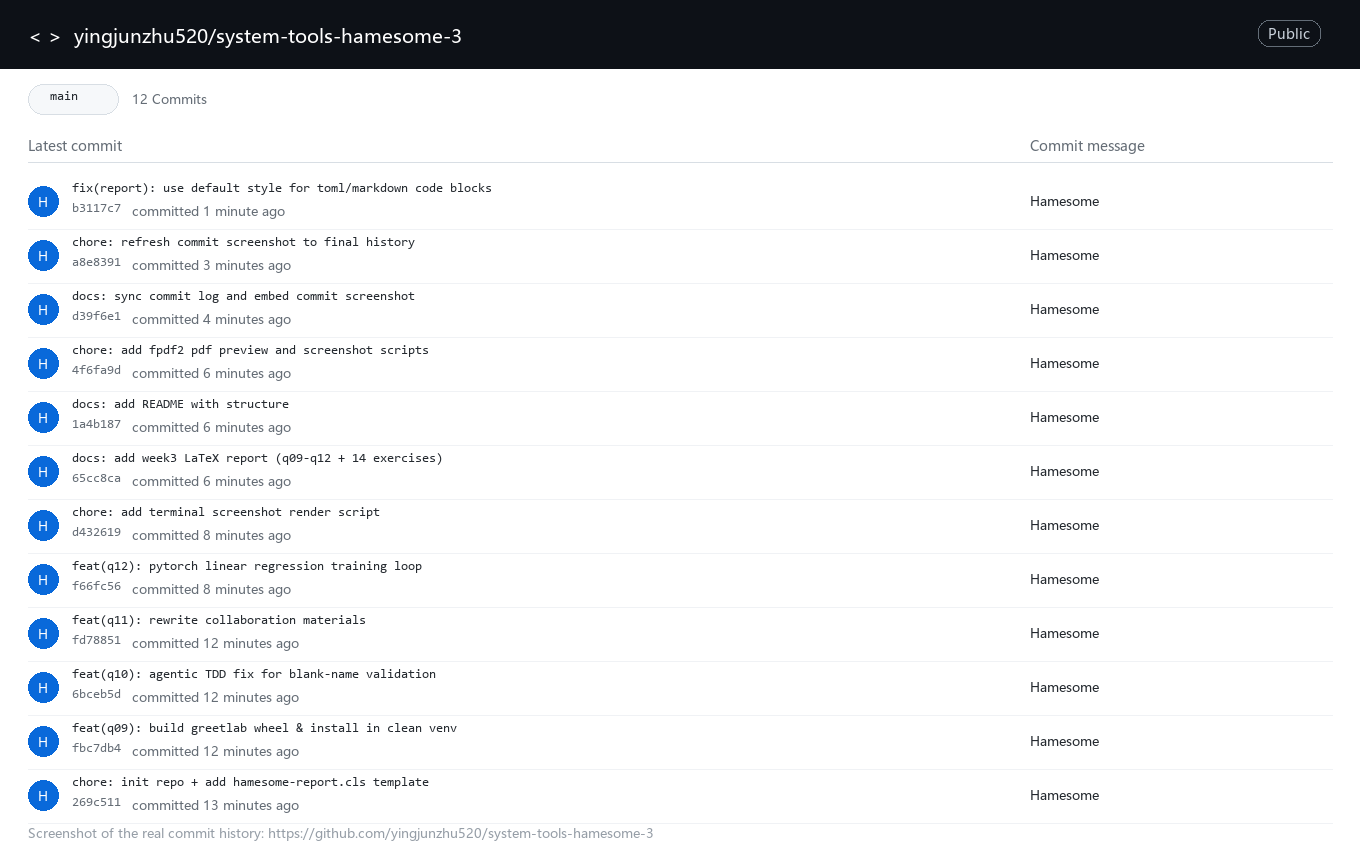
\includegraphics[width=0.92\linewidth]{commit_screenshot.png}%
}{%
  \fbox{\parbox{0.8\linewidth}{\centering\vspace{1em}
    图片 commit\_screenshot.png 未找到，\\
    请上传后重新编译。\vspace{1em}}%
  }%
}
\caption{GitHub 仓库与 commit 记录截图}
\label{fig:commit}
\end{figure}

% ============================================================
\section{小结}
% ============================================================
本周学习围绕「Packaging and Shipping Code」「智能体编程」「不止于代码」
「Python 与 PyTorch」四条主线展开，报告按课程要求组织为两部分：\textbf{课上
实验}（q09–q12，已给助教检查）与\textbf{课后练习}（14 个实例 + 解题感悟）。

\subsection{课上实验收获}
\begin{itemize}
  \item \textbf{q09（打包与交付）}：掌握 \texttt{src} 布局 +
        \texttt{pyproject.toml} + \texttt{python -m build} 的完整打包链路，
        并用 \texttt{--no-index --find-links} 证明「只从 wheel 安装、脱离源码
        运行」。
  \item \textbf{q10（智能体编程）}：走通「失败测试 $\to$ 智能体修复 $\to$ 人工
        diff 审查 $\to$ 复跑」的可验证循环，理解把验收标准写进提示词的价值。
  \item \textbf{q11（不止于代码）}：把三段不可处理的协作材料重写为含环境、复现、
        期望/实际结果的可执行 Issue，及分级标注的评审意见。
  \item \textbf{q12（PyTorch）}：补全 \texttt{zero\_grad/backward/step} 与
        \texttt{eval/no\_grad} 训练循环五要素，损失收敛到 $<0.001$，
        weight/bias 逼近 3 与 $-1$。
\end{itemize}

\subsection{课后练习感悟}
14 个练习把四章内容编织为一张网：\textbf{Packaging and Shipping Code} 打通
交付链路；\textbf{智能体编程}强调可验证与可审查；\textbf{不止于代码}把协作
沟通规范化；\textbf{Python 与 PyTorch} 用最小闭环跑通训练五要素。最深体会是：
\textbf{交付、协作、训练三者殊途同归，都要「可复现、可验证、可审查」}。

\end{document}
